% This is samplepaper.tex, a sample chapter demonstrating the
% LLNCS macro package for Springer Computer Science proceedings;
% Version 2.20 of 2017/10/04
%
\documentclass[runningheads]{llncs}
%
\usepackage{graphicx}
% Used for displaying a sample figure. If possible, figure files should
% be included in EPS format.
%
% If you use the hyperref package, please uncomment the following line
% to display URLs in blue roman font according to Springer's eBook style:
% \renewcommand\UrlFont{\color{blue}\rmfamily}
\usepackage{url}
\def\UrlBreaks{\do\/\do-}
\usepackage{breakurl}
\usepackage[breaklinks]{hyperref}

\begin{document}
%
\title{Application of Computer Vision in Robotics}
%
%\titlerunning{Abbreviated paper title}
% If the paper title is too long for the running head, you can set
% an abbreviated paper title here
%
\author{Jenny Rudnitskiy}
%
%\authorrunning{F. Author et al.}
% First names are abbreviated in the running head.
% If there are more than two authors, 'et al.' is used.
%
\institute{Centre for Research in Mathematics and Data Science, Western Sydney University
\email{19892274@student.westernsydney.edu.au}}
%
\maketitle              % typeset the header of the contribution
%
\begin{abstract}
In this paper we propose Bird-watching Robot on the basis of the Raspberry Pi 4 Computer Model B (8GB RAM), using one Raspberry Pi Camera V2 and Pimoroni pan-tilt HAT for object tracking. The rpi-deep-pantilt software package developed using convolutional neural networks and transferred learning technique is used for object detection and classification.  


\keywords{robotics  \and artificial intelligence \and raspberry pi.}
\end{abstract}
%
%
%
\section{Computer Vision in Robotics}
\subsection{Project Objective and Challenges}
\setlength{\parskip}{1em}
Artificial Intelligence is increasingly occupying big part in our everyday life: from voice-to-text technology like Google Assistants, chatbots to autonomous self-driving vehicles and drone surveillance. However robotics is still somewhere behind this trend with countries like Japan leading in the field of robot technology but not Australia. When speaking of the robots, we imagine industrial machines that are used to automate the processes and substitute physical human labour, in the household environment we imagine vacuum cleaners like 'iRobots'. But can we think of robots as indispensable part of our life? In this paper we propose a object detection robotic solution that can be easily integrated into everyday life of someone who loves bird-watching.

Object detection is a complicated task that not only predicts the object but also its location in terms of bounding boxes and requires significant amount of data to train deep learning algorithms and processing power. The challenge that we faced was to design a low-cost robotic solution that can be used for object detection and tracking on a small device in everyday life. The combination of Raspberry Pi hardware and rpi-deep-pantilt software package allowed us achieving this. The rpi-deep-pantilt package is one of very few packages that currently exist. It combines a single-shot detector (a type of convolutional neural network), PID controller and pi-camera  and is specifically designed for use on a small light-weight device like Raspberry Pi. 

In the context of this project it would be useful to explain the difference between robot vision and computer vision. At its core, Robot Vision is a combination of algorithms, cameras and hardware components that work unanimously in order to provide visual insights to the robot or machine. This helps the robot to accomplish complex tasks that require visual understanding.

Computer Vision aims on rendering advanced visual capabilities to the computers by means of complex algorithms and camera hardware. It mainly deals with image recognition. The computer vision methods initially extract useful information from the digital images and videos. This information is then processed and analysed.\cite {ref_url1} 

\subsection{Application of Convolutional Neural Networks in Object Detection} 

With the significant advancement of deep learning models, the CNN models have demonstrated 'superhuman performance'\cite{ref_book} and became the go-to models for image search services, self-driving cars, automatic video classification, voice recognition, and natural language processing (NLP). Their performance can be assessed both in terms of accuracy and capturing spatial invariance. With real-time object detection and tracking, CNN allows to achieve same result under minor shifts, rotations and deformations. Other networks would have to learn the pattern all over again if it appeared in a new location.\cite {ref_article1}  		

The object detection is done using SSD MobileNetV3 model. It was pre-trained on Common Objects in Context (COCO) dataset and converted to TensorFlow Lite.

\subsection{SSD Architecture} 

\begin{figure}[hbt!]
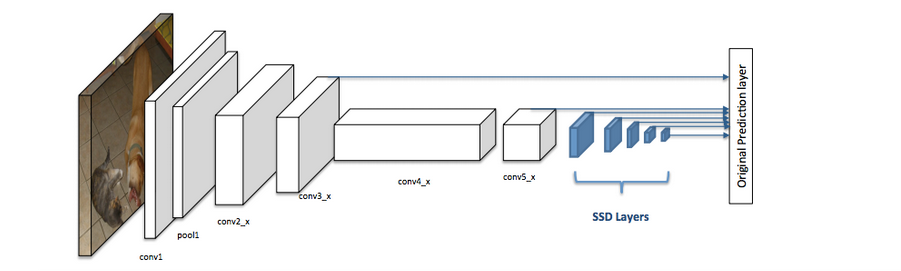
\includegraphics[width=\textwidth]{SSD_Mobilenet.png}
\caption{Architecture of Convolutional Neural Network with the Single-Shot Detector.} \label{fig1}
\end{figure}

SSD has two components: a backbone model and SSD head. Backbone model usually is a pre-trained image classification network as a feature extractor. In our case it is MobileNetV3 pretrained on  COCO dataset  from which the final fully connected classification layer has been removed. A deep neural network is left that is able to extract semantic meaning from the input image while preserving the spatial structure of the image albeit at a lower resolution. For MobileNetV3, the backbone results in a 320X320 resolution 1x1 feature map for an input image. The SSD head is just one or more convolutional layers added to this backbone and the outputs are interpreted as the bounding boxes and classes of objects in the spatial location of the final layers activations.\cite {ref_url2}


\section{Bird Robot Hardware}

Bird robot hardware can be divided into the following sets: 
\begin{description} 
 \item[$\bullet$ Raspberry Pi] 
 \item \noindent A small size fully-functional computer that can be programmed almost in any language, and to which additional hardware can be attached. 
 \begin{figure}[hbt!]
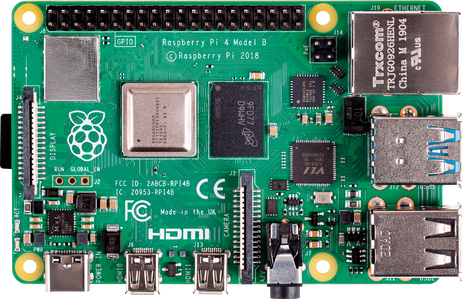
\includegraphics[width=\textwidth]{rasp_pi_4_b_03_anw.png}
\caption{Raspberry Pi 4 Computer.} \label{fig1}
\end{figure}
  \item[$\bullet$ Pi Camera] 
 \item\noindent For this project we use the 8-megapixel camera module attached to Raspberry Pi board with the help of a ribbon cable that gives our robot the ability to see. Pi Camera is able to provide 1920x1080 pixels resolution for up to a rate of 30 frames per second (FPS).
 
 \begin{figure}[hbt!]
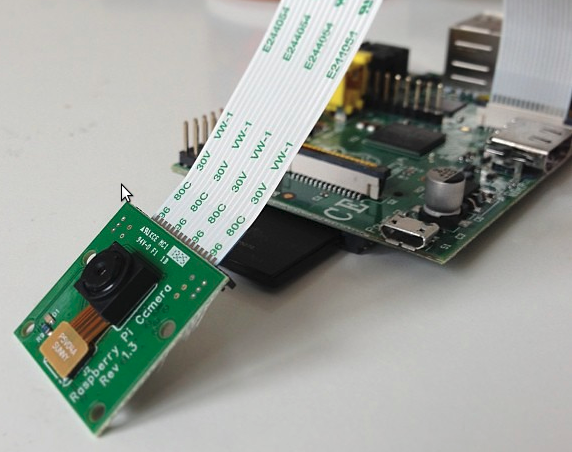
\includegraphics[width=\textwidth]{Pi camera.png}
\caption{Pi Camera.} \label{fig1}
\end{figure}
 \item[$\bullet$ Pan-Tilt HAT]
  \item\noindent The HAT and its on-board microcontroller allow independently drive the two servos (pan and tilt). The module pans and tilts through 180 degrees in each axis.\cite{tech_doc}
\end{description}

\section{PID Controller and Object Tracking}
PID Control stands for Proportional-Integral-Derivative feedback control and is of the most commonly used controllers in robotics. The PID Controller bases its functionality on computation of 'tracking error' $e$ and its three gains $K_P$, $K_I$ and $K_D$. 
In the combination they lead to the control action $u$, as shown in the following expression:

\begin{equation}
u(t) = K_P e(t) +  K_I\int e(t)dt + K_D\frac {de(t)}{dt}
\end{equation}

\item\noindent The proportional term corresponds to the first part of the expression, the integral action to the second, and the derivative to the last one. 
\item\noindent Each action of the PID components plays its own role and requires tuning in combination. One cannot independently tune the three different gains, as each of them offers the desired response characteristics but at the same time has a negative effect that has to be compensated by re-tuning another gain.\cite{ref_url3}

\item\noindent The following three characteristics indicate that the system is properly tuned: response time, settling time and overshoot. The goal of tuning is to minimise response time, settling time and overshoot.

\begin{figure}[hbt!]
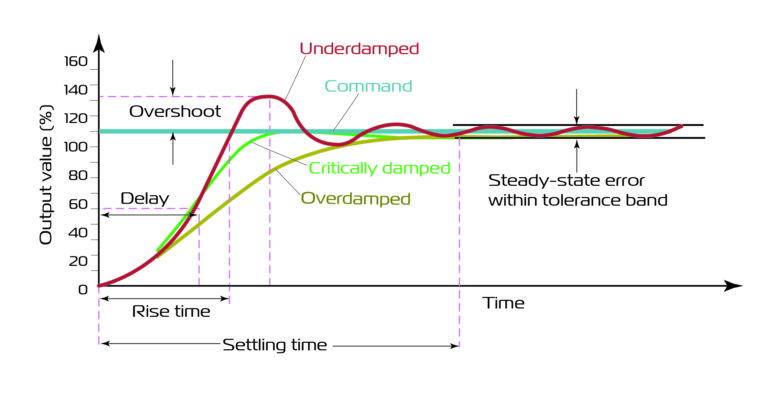
\includegraphics[width=\textwidth]{Motion_Controller.jpg}
\caption{Values to evaluate control systems.} \label{fig1}\cite{ref_url4}
\end{figure}

\item\noindent In our case PID tuning ensures tracking the object smoothly that the camera stays centered upon an object. 
To accomplish this goal the following four processes are programmed\cite{ref_url5}:
\begin{itemize}
 \item A process that finds the object in the frame,
 \item A process that calculates panning angles with PID,  
 \item A process that calculates tilting angles with PID, and
 \item A process that drives the servos.
\end{itemize}

Due to the use of the CNN (even after conversion to  Tensorflow Lite) for object detection and classification the PID object tracking becomes extremely slow and the use of Google Coral TPU USB Accelerator is recommended. 


\section{Conclusions} 
In this project we attempted to build a bird detecting robot using a combination of machine learning software and hardware. The CNN, the neural network widely used in computer and robotic vision, computational complexity is overcome by implementing pre-trained model (MobileNetV3 SSD). The performance of model on unseen video streaming data was impressive, cockatoos and crested pigeons were detected and classified as birds. 

%
% ---- Bibliography ----
%
% BibTeX users should specify bibliography style 'splncs04'.
% References will then be sorted and formatted in the correct style.
%
% \bibliographystyle{splncs04}
% \bibliography{mybibliography}
%

\begin{thebibliography}{8}

\bibitem{ref_url1}

Computer Vision vs Robot Understanding the Difference, \url{https://www.oodlestechnologies.com/blogs/computer-vision-vs-robot-vision-understanding-the-difference/}. 
Last accessed 20 Feb 2021

\bibitem{ref_book}

Pradeep Pujari, Mohit Sewak, Md. Rezaul Karim
{\it Practical Convolutional Neural Networks},
Published by Packt Publishing,
2018.

\bibitem{ref_article1}

Cynthia R., David C.: The Secrets of Machine Learning: Ten Things
You Wish You Had Known Earlier to be More Effective at Data Analysis. Tutorials in Operation Research \textbf, p.9 (2019)


\bibitem{ref_url2}
How single-shot detector (SSD) works,
\url{https://developers.arcgis.com/python/guide/how-ssd-works/}. 
Last accessed 20 Feb 2021


\bibitem{tech_doc}
Pimoroni Pan-Tilt HAT Latest Documents,
https://pantilt-hat.readthedocs.io/en/latest/. 
Last accessed 21 Feb 2021

\bibitem{ref_url3}
PID Control,
\url{https://www.autonomousrobotslab.com/pid-control.html/}. 
Last accessed 20 Feb 2021

\bibitem{ref_url4}
How to address overshoot in servo control, by Danielle Collins, October 2017
\url{https://www.motioncontroltips.com/how-to-address-overshoot-in-servo-control/}. 
Last accessed 20 Feb 2021


\bibitem{ref_url5}
Pan/tilt face tracking with a Raspberry Pi and OpenCV, April 2019
\url{https://www.pyimagesearch.com/2019/04/01/pan-tilt-face-tracking-with-a-raspberry-pi-and-opencv/}. 
Last accessed 20 Feb 2021

\end{thebibliography}
\end{document}


